\chapter{Background}


Understanding the idealized cosmological expansion model, as well as the deviations in motion from it, requires detailed spectroscopic and photometric measurements of galaxies, Cepheid variable stars, and supernovae type Ia. Those measurements, however, are readily available and have been calibrated and expanded by numerous sources. In this section I will provide the precursory background knowledge on how these measurements came about and how they lead to an idealized cosmological expansion model. Then I will show how deviations appear within the model that we can use to trace the large scale motion we are interested in understanding.


\subsection{Measuring Redshift through Spectroscopy}

Since each atom has a unique spectrum composed of emission and absorption line, astronomers use spectroscopic measurements to determine useful information such as the composition and velocity of astronomical objects. This is accomplished by comparing the position of the spectral lines of hydrogen observed in astronomical objects to those measured in a rest frame where the object is not moving with respect to the Earth. The result is an observed shift towards longer, "redder" wavelengths (see Fig. \ref{fig:redshift}) \cite{SpectralRedshift}. This phenomenon called the redshift is calculated using the Doppler effect, which is a means of measuring the shift in the spectral lines due to motion away from the point of observation:
%
\begin{equation}\label{ds}
z \equiv \frac{\lambda_{o}}{\lambda_{r}} -1 = \frac{\Delta \lambda}{\lambda_{r}}
\end{equation}
%
where $z$ is the redshift, $\lambda_{o}$ is the spectral line as observed from the astronomical object, $\lambda_{r}$ is the spectral line as measured at rest on Earth, $\Delta \lambda$ is the shift between $\lambda_{o}$ and $\lambda_{r}$ \cite{Hogg1999:DistanceMeas+GenRef}\cite{moore2012general}. We can relate the redshift to the velocity of the object receding away from us through the relativistic Doppler effect as follows:
%
\begin{equation}\label{rds}
z = \sqrt{\frac{1+v/c}{1-v/c}} - 1
\end{equation}
%
where $v$ is the line-of-sight radial velocity of the object and $c$ is the speed of light \cite{Hogg1999:DistanceMeas+GenRef}\cite{Kirshner2004:HubbleDiagram}\cite{moore2012general}. And, in the limiting case where the radial velocity is much less than the speed of light, the equation reduces to
%
\begin{equation}\label{redshift-radialvelo}
z \approx \frac{v}{c}
\end{equation}
%
which is the relationship used to relate the redshift in the spectral lines to the radial velocity of a galaxy \cite{Hogg1999:DistanceMeas+GenRef}\cite{moore2012general}.


\begin{figure}[t]
	\centering
	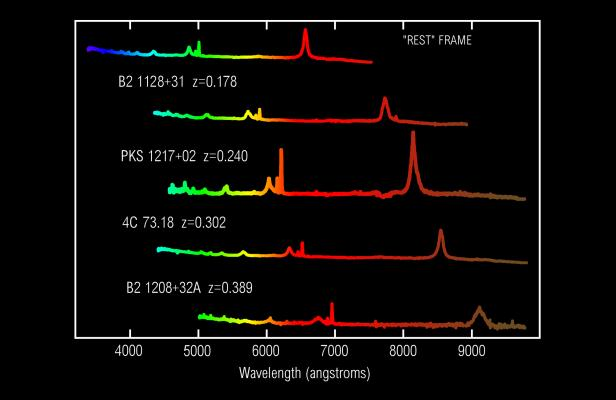
\includegraphics[width=\textwidth]{redshift}
	\caption{Hydrogen Spectra of Quasi-Stellar Objects (QSO) Exhibiting Redshift \cite{SpectralRedshift}. The first spectrum is an example of a QSO in a theoretical "rest frame" with no motion with respect to Earth. The subsequent spectra are of four different QSOs in order of increasing velocity away from Earth. As velocity increases there is a corresponding increase in redshift $z$ from the rest frame. While the hydrogen lines shift to longer, ``redder" wavelengths, the spacing in the spectral lines remains the same between spectra \cite{SpectralRedshift}.}
	\label{fig:redshift}
\end{figure}

\subsection{Measuring Distance through Luminosity}


The most precise method of measuring distance to a galaxy is by measuring the luminosity of Type Ia supernovae \cite{Branch1992:SNeIa+StandardCandles}\cite{Goobar1995:StandardCandles}. However, supernova Type Ia are quite rare as they are only known to occur around once every hundred year in a galaxy. The reason that Type Ia supernovae are often sought after and used as standard candles of distance is due to the fact that they only occur when a white dwarf star explodes from accruing mass until it has reached its maximum size of 1.44 solar masses, known as the Chandrasekhar limit. After this point, the star will suddenly explode in a highly predictable manner as a Type Ia supernova \cite{Carroll2001-CosmoReview+SNeIa+Lum}\cite{Krisciunas2005:SNeIa}\cite{Narayan2016:SNeIa+Redshift}. This is because we know that all white dwarfs must overcome a critical mass in order for a supernova to occur; therefore, models have been used to accurately predict the behavior of the explosion based on the principle that nearly all Type Ia supernova begin roughly at the same mass, size, and composition \cite{Goobar1995:StandardCandles}. Using photometry we can measure the apparent magnitude or the brightness as seen on Earth over time, otherwise known as the light curve, of a Type Ia supernova. From the models we can usually accurately predict the luminosity or absolute magnitude of a Type Ia supernova, which is a standard measurement of the brightness of an object as seen from 10 parsecs away \cite{Reiss2007:SNeIa}. Given these measurements we can calculate the luminosity distance $D_L$ of a Type Ia supernova from the distance modulus equation:
%
\begin{equation}\label{dm}
m = M + 5 \log [D_L] + K + 25
\end{equation}
%
where $m$ is the apparent magnitude, $M$ is the absolute magnitude, and $K$ is a correction term due to redshifting \cite{Carroll2001-CosmoReview+SNeIa+Lum}\cite{Narayan2016:SNeIa+Redshift}.



\subsection{Hubble's Law and Hubble constant}



Given measurements of the redshift and distances from Type Ia supernova surveys, astronomers can plot the radial velocity as a function of distance as seen in Fig. \ref{fig:TypeIa} \cite{Kirshner2004:HubbleDiagram}. Again, using the limiting case where the radial velocity $v$ is much less than $c$, we can write the relationship seen in Fig. \ref{fig:TypeIa} as
%
\begin{equation}\label{hubblelaw}
cz \approx v = H_0 r
\end{equation}
%
where we have chosen to rewrite the luminosity distance $D_L$ as the radial distance $r$ away from us, $z$ is the redshift, and $H_0$ is a proportionality constant between the receding radial velocity and the distance to that object. Eq. \ref{hubblelaw} is known as Hubble's Law, after the astronomer Edwin Hubble who initially discovered this relationship \cite{Kirshner2004:HubbleDiagram}. The proportionality constant $H_0$ is the Hubble constant with units of inverse time, but is most usefully written as
%
\begin{equation}\label{hubbleconst}
H_0 = 100\,h\;\, km\, s^{-1}\, {Mpc} ^{-1}
\end{equation}
%
where $h$ is a dimensionless parameterization constant depending on current measurements. Hubble's Law states that as you increase in distance you have a corresponding increase in radial velocity (and therefore redshift) of the objects observed. The importance of the Hubble constant is that it emphasizes the constant rate of increase in the graph as the rate of change of space (or "stretching") in ${km}/{s}$ per megaparsec of space \cite{Hogg1999:DistanceMeas+GenRef}\cite{Kirshner2004:HubbleDiagram}. This may seem odd, but Eq. \ref{redshift-radialvelo} and Eq. \ref{hubblelaw} state that with increasing radial velocity and distance there is also a corresponding increase in the observed redshift, which is due to further objects having traveled longer through a stretching space. Thus, the Hubble constant $H_0$ measures the current rate of expansion of the universe.

\begin{figure}[h]
	\centering
	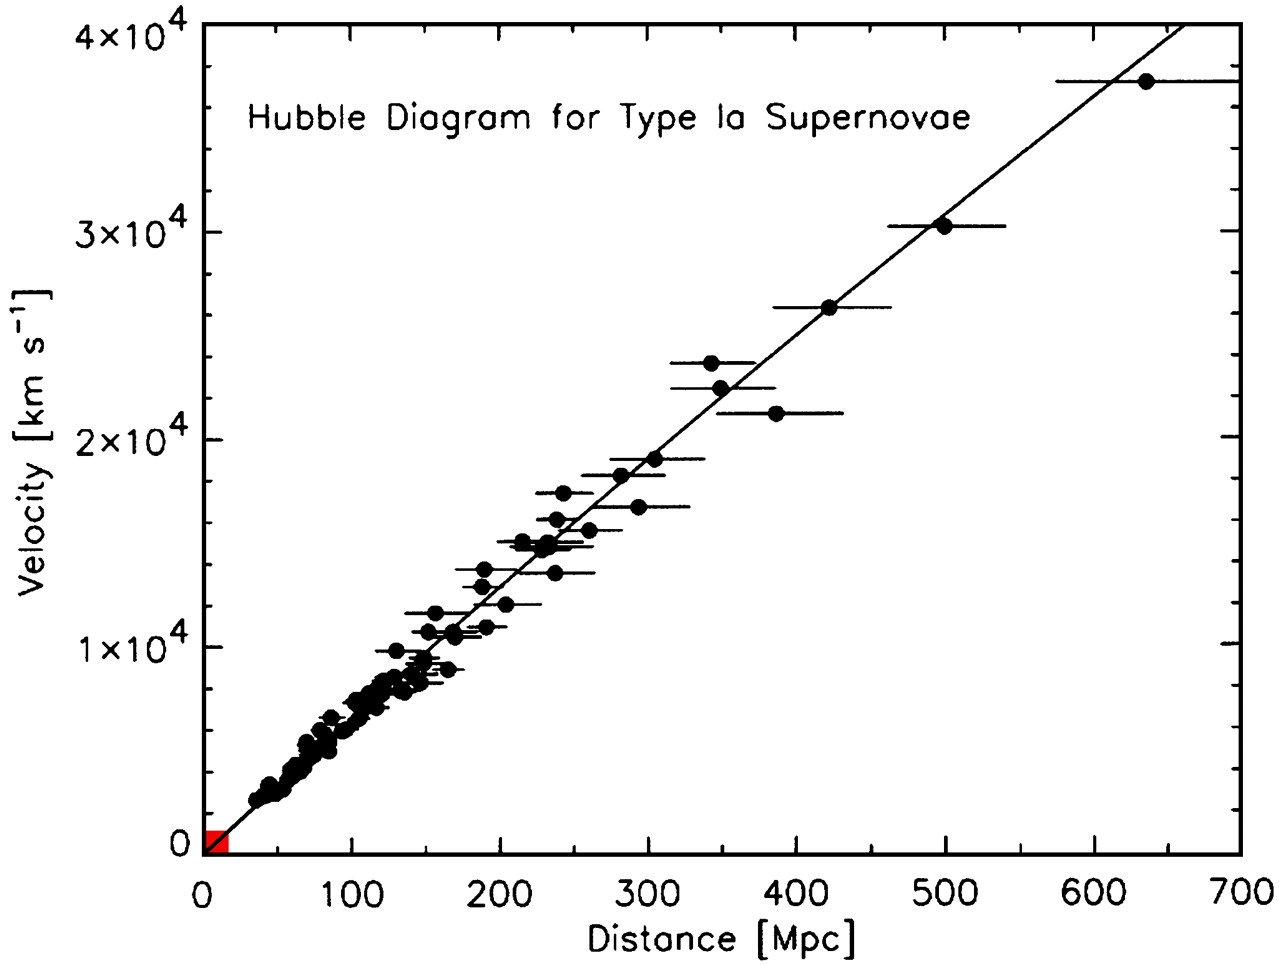
\includegraphics[width=0.75\textwidth]{TypeIa}
	\caption{Hubble Diagram for Type Ia Supernovae  \cite{Kirshner2004:HubbleDiagram}. The linear relationship between velocity and distance is described by Hubble's law, where the slope is the Hubble constant $H_0$ in $km\, s^{-1}\, {Mpc}^{-1}$. The scatter in the distance is associated with a statistical error of $<10\%$ per object measured, with the error increasing with distance. The small red box in the bottom left corner corresponds to the window size of Edwin Hubble's original measurements in 1929.}
	\label{fig:TypeIa}
\end{figure}

Efforts to accurately measure the Hubble constant are significantly improved by standard candles like Type 1a supernovae (as seen in Fig. \ref{fig:TypeIa}), but due to their rarity these measurements must be combined with other methods to improve the overall value of $H_0$ \cite{Narayan2016:SNeIa+Redshift}\cite{Riess2016:H0+2.4}\cite{Kaiser2015:PerturbLumDist+PecVelo}\cite{Reiss2007:SNeIa}.  Estimates place bounds on the Hubble parameter $h$ within the range of $0.65$ and $0.8$, while recent progress in measuring $H_0$ by Riess et al. (2016) give an estimate of $73.24\ \pm\ 1.74$ $km s^{-1} Mpc^{-1}$ with a 2.4\% uncertainty in the measurement \cite{Riess2016:H0+2.4}. For challenges and tension in estimating the current Hubble constant I encourage the reader to review Jos\'e Luis Bernala et al. (2016), ``The trouble with $H_0$", for a more comprehensive overview outside the scope of this thesis \cite{Bernal2016:Trouble+H0}.


\subsection{Peculiar Velocity}

The relationship described by Hubble's Law in Eq. \ref{hubblelaw} is a model for an idealized isotropic cosmological expansion where galactic objects are stationary with only relative motion due to expansion \cite{Hogg1999:DistanceMeas+GenRef}. From this ideal model you can then estimate the redshift solely due to expansion, known as the cosmological redshift, from $z_{cos}\equiv z={{H_0r}/c}$. This model, however, neglects the intrinsic motion of galaxies due to gravitational attraction and/or residual momentum gained from the Big Bang \cite{Feldman2008}\cite{Watkins2007}. These are seen as fluctuations in the radial velocity about the ideal expansion line in Fig. \ref{fig:TypeIa} as expressed by an ideal Hubble's law. The deviations in the observed redshift from the ideal expansion model are actually measurements of the Doppler redshift due to intrinsic galactic motion \cite{Hogg1999:DistanceMeas+GenRef}\cite{Carroll2001-CosmoReview+SNeIa+Lum}. We can account for the deviations in Hubble's law as an additional velocity term due to the intrinsic motion such that
%
\begin{equation}
cz_{obs} = H_0 r + v_p
\end{equation}
%
where $z_{obs}$ is the observed redshift and $v_p$ is the \textit{peculiar velocity}, where peculiar implies intrinsic or unique to that object. The peculiar velocity $v_p$ of an astronomical object can be calculated from
%
\begin{equation}\label{pecvelo-redshift}
v_p = \frac{c\,(z_{obs} - z_{cos})}{(1+z_{cos})}
\end{equation}
%
where $z_{obs}$ is the observed redshift and $z_{cos}$ is the cosmological redshift \cite{Hogg1999:DistanceMeas+GenRef}. Using the idealized form of Hubble's law from Eq. \ref{hubblelaw} we can include the distance $r$, since $z_{cos}$ is not directly observable, such that Eq. \ref{pecvelo-redshift} can be rewritten as
%
\begin{eqnarray}
v_p = \frac{cz_{obs} - {H_0\, r}}{1+{H_0\, r}/c} \approx \frac{cz_{obs} - H_0\, r}{1+z_{obs}}
\end{eqnarray}
%
where we have made the (reasonable) assumption that $v_p \ll H_0 r$ such that $z_{obs} \approx z_{cos}$. \cite{Watkins2015:BulkFlow+CF2}\cite{Watkins2015:UnbiasedEstimator}.
However, Eq. \ref{pecvelo-redshift} is a useful tool for visualizing how we discriminate between cosmological redshift and the Doppler redshift in peculiar velocity calculations.



\subsection{Cosmic scales}


An important limitation on Hubble's law from Eq. \ref{redshift-radialvelo} states that the radial velocity must be much less than the speed of light. Since the radial velocity is the sum of the cosmological expansion $H_0\, r$ and the peculiar velocity $v_p$, this places a few limitations on the quantities we can calculate. This is because we know that the radial velocity is proportional to the redshift in the spectra of a distant object, and thus if the observed redshift becomes too large then the approximation held by Eq. \ref{redshift-radialvelo} is no longer valid. Such calculations at high redshifts using this method thus inherently introduce distortions in the radial velocity, with estimates placing the limit on the redshift at $z < 2$ before corrections are needed \cite{Kaiser2015:PerturbLumDist+PecVelo}. Since radial velocity is also proportional to the distance of an object, the same reasoning can be used to set limits on the distance. Fortunately, in this thesis we will be working with scales well within the boundaries of $v \ll c$ and $z < 2$. I define these scales below explicitly in terms of distance and size.



On very small scales, on the order of magnitude of individual galaxies ($\mytilde 10\ kpc$) the motion due to cosmic expansion is small compared to the peculiar motion. At this scale, the motion that dominates is due to gravitational attraction pulling objects towards regions of higher density. Even at small scales of the size of clusters ($\mytilde 5\; h^{-1}\, Mpc$), motion towards regions of higher density dominate such that peculiar motion of a cluster tends to be on the same scale as the cosmic expansion. At the larger scales that we are interested in ($\mytilde 100\; h^{-1}\, Mpc$), you can think of the Earth as being at the center of an immense sphere with a multitude of clusters and individual galaxies moving around with their own peculiar velocities. At this scale, the motion is almost entirely dominated by the cosmic expansion with the sphere having a very small peculiar motion (a sum of all the motion within the sphere) known as the bulk flow \cite{Feldman2008}\cite{Watkins2015:BulkFlow+CF2}. The bulk flow provides us with great insight into the origin and evolution of our universe through the directionality and motion \cite{Watkins2007}\cite{Watkins2009:LCDM+Challenge}\cite{Macaulay21092012}. In thesis we will be concerning ourselves with radial and peculiar velocity measurements relative to these scales.

\begin{figure}[h]
	\centering
	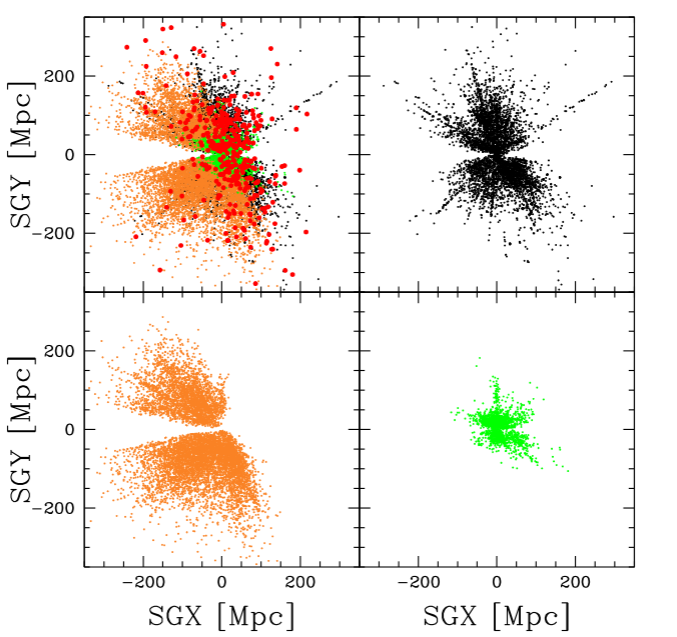
\includegraphics[width=\textwidth]{CF3}
	\caption{Distances of Individual Galaxies in the \textit{Cosmicflows-3} (CF3) Database Projected on Supergalactic SGX-SGY planes  \cite{Tully2016:cf3}. Upper right: distances from the precursor \textit{Cosmicflows-2} compendium in black \cite{Tully2013:cf2}, Bottom Left: distances from Six Degree Field Galaxy Survey (6dFGS) of the Fundamental Plane in orange, Bottom Right: distances from the Splitzer Space Telescope infrared measurements of galaxy rotation in green. Upper left: all galaxies from different measurement surveys included in CF3 projected on one plane as well as distance measurements from Type 1a supernovae in red.}
	\label{fig:CF3}
\end{figure}


\subsection{\textit{Cosmicflows-3} Database}


For our study of peculiar velocities we will be using distance measurements from the \textit{Cosmicflows-3} (CF3) compendium, which is a collection of various observational surveys of 17,669 individual galaxies (see Fig. \ref{fig:CF3}) \cite{Tully2016:cf3}. Each galaxy distance is measured and calibrated amongst different sources and surveys such as Type Ia supernovae observations, infrared photometry of galaxy rotation,  Cepheid variables photometry, and estimating the tip of the red giant branch. The galaxies are organized into groups of similar distances; for example, the Virgo Cluster, the largest group, consists of 161 individual galaxy measurements. The compendium provides 11,508 groups organized in this manner, but nearly every group contain less than ten galaxies and 9804 groups are denoted as "singles" due to containing only one galaxy. Despite the limited amount of groups with more than two galaxies, this is a significant improvement to its predecessor \textit{Cosmicflows-2} which contained only 8,188 individual galaxy entries in total \cite{Tully2013:cf2}. The distances (and the observed redshift) provided by \textit{Cosmicflows-3} allows us to calculate the peculiar velocity for both individual galaxies as well as groups.
